\begin{document}
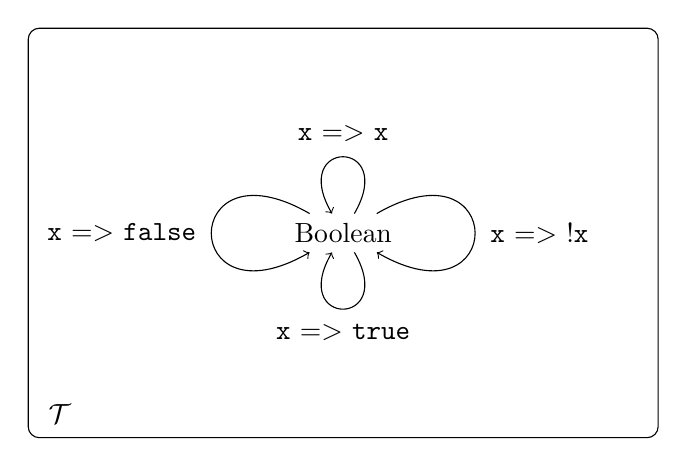
\begin{tikzpicture}
  \draw[rounded corners] (-4,-2.6) rectangle (4,2.6);
  \node at (-3.6,-2.3) {$\mathcal{T}$};
  \node (B) at (0,0) {$\mathrm{Boolean}$};
  \draw[->] (B) to[out=60,in=120,looseness=10] node[above=2pt] {$\mathtt{x\ {=}{>}\ x}$} (B);
  \draw[->] (B) to[out=30,in=-30,looseness=10] node[right=2pt] {$\mathtt{x\ {=}{>}\ !x}$} (B);
  \draw[->] (B) to[out=-60,in=-120,looseness=10] node[below=2pt] {$\mathtt{x\ {=}{>}\ true}$} (B);
  \draw[->] (B) to[out=150,in=210,looseness=10] node[left=2pt] {$\mathtt{x\ {=}{>}\ false}$} (B);
\end{tikzpicture}
\end{document}
